%%%%% Diagnosing Thoracic Diseases Using Machine Learning & Medical Imaging

\documentclass{article}

\usepackage{microtype}
\usepackage{graphicx}
\usepackage{subfigure}
\usepackage{subcaption}
\usepackage{caption}
\usepackage{booktabs}
\usepackage[%  
    colorlinks=true,
    pdfborder={0 0 0},
    linkcolor=red
]{hyperref}

\newcommand{\theHalgorithm}{\arabic{algorithm}}
\usepackage[accepted]{icml2024}

\usepackage{amsmath}
\usepackage{amssymb}
\usepackage{mathtools}
\usepackage{amsthm}

\usepackage[capitalize,noabbrev]{cleveref}

\graphicspath{{./Images}}

%%%%%%%%%%%%%%%%%%%%%%%%%%%%%%%%
% THEOREMS
%%%%%%%%%%%%%%%%%%%%%%%%%%%%%%%%
\theoremstyle{plain}
\newtheorem{theorem}{Theorem}[section]
\newtheorem{proposition}[theorem]{Proposition}
\newtheorem{lemma}[theorem]{Lemma}
\newtheorem{corollary}[theorem]{Corollary}
\theoremstyle{definition}
\newtheorem{definition}[theorem]{Definition}
\newtheorem{assumption}[theorem]{Assumption}
\theoremstyle{remark}
\newtheorem{remark}[theorem]{Remark}

\usepackage[textsize=tiny]{todonotes}

\icmltitlerunning{Diagnosing Thoracic Diseases Using ML}

\begin{document}

\twocolumn[
\icmltitle{Diagnosing Thoracic Diseases Using Machine Learning and Medical Imaging}

\begin{icmlauthorlist}
\icmlauthor{Wendy Carvalho (02026116),}{}
\icmlauthor{Meriem Elkoudi (02015993),}{}
\icmlauthor{Chris Peters (01989716),}{}
\icmlauthor{Saim Siddiqui (02018510),}{}
\icmlauthor{and Amitha Thalanki (02077527)}{}
\end{icmlauthorlist}

\vskip 0.3in
]

%%%%%%%%%%%%%%%%%%%%%%%%%%%%%%%%
% ABSTRACT
%%%%%%%%%%%%%%%%%%%%%%%%%%%%%%%%

\begin{abstract}

This project explores how machine learning can be used in medical imaging to diagnose thoracic
diseases such as pneumonia, emphysema, and fibrosis. It utilizes a curated subset of 810
high-quality, radiologist-verified chest X-ray images from the NIH ChestX-ray8 dataset in which
three models were developed to attempt to diagnose patients. The models that were used were a Support
Vector Machine and two Convolutional Neural Networks, ResNet50 and MobileNet. The SVM achieved
moderate accuracy but was limited by computational expense. ResNet50 demonstrated high recall,
identifying many true positives but over-predicted diseases, while MobileNet achieved 89\% binary
accuracy and was the best model. The results show the great potential of machine learning in the
medical field, especially in diagnostics offering tools to assist clinicians and improve patient
outcomes.

\end{abstract}

%%%%%%%%%%%%%%%%%%%%%%%%%%%%%%%%
% INTRODUCTION
%%%%%%%%%%%%%%%%%%%%%%%%%%%%%%%%

\section{Introduction}
Thoracic diseases, including pneumonia, emphysema, and fibrosis, are common causes of morbidity and
mortality worldwide. Chest X-rays are one of the most widely accessible and commonly used diagnostic
tools for detecting these conditions. However, interpreting these images is complex, and clinical
diagnoses are often challenging, even for experienced radiologists.

Machine learning techniques are used to address this challenge by enabling automated analysis of
medical images. Bringing this leading-edge technology's immense power into the diagnostics field can
potentially increase the capacity for trained professionals to diagnose patients properly, sooner,
and in more difficult-to-identify cases.

This project aims to build a computer-aided diagnostic (CAD) tool capable of diagnosing thoracic
diseases from chest X-ray images, assisting clinicians by automating the detection of common thoracic
diseases. This has been implemented using Support Vector Machines (SVM) and Convolutional Neural Networks
(CNN) in the form of ResNet50 and MobileNet. The efficacy of all are tested.

%%%%%%%%%%%%%%%%%%%%%%%%%%%%%%%%
% DATA
%%%%%%%%%%%%%%%%%%%%%%%%%%%%%%%%

\section{Data}
The data for this project has been obtained from the NIH ChestX-ray8 dataset, an open-source,
hospital-scale collection of medical images, which will be essential for developing a CAD system.
The original NIH ChestX-ray8 dataset contains 108,948 images from 32,717 patients, however, the
labels are frequently incorrect and misdiagnoses.
A subset of 810 images was chosen based on the evaluation of radiologists themselves. The 810 image
subset is the only commonly known verified chest X-ray dataset. Each image is high-resolution
(1024x1024 px) and in PNG format.

Figure \ref{fig:examplexray} shows an example X-ray from the dataset, with the diagnoses of
Atelectasis, Effusion, and Pneumothorax. As shown, each individual X-ray can have multiple labels
associated with it, which further complicates the dataset.

%%% EXAMPLE X-RAY IMAGE %%%
\begin{figure}[!h]
    \centering
    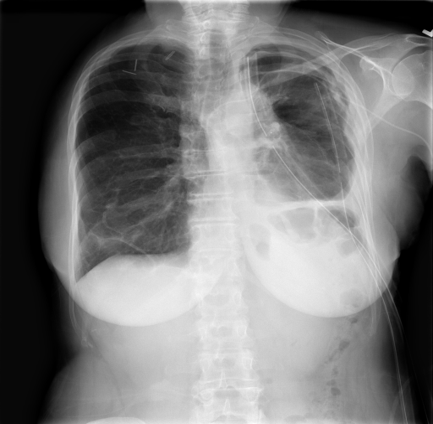
\includegraphics[scale=0.5]{00018366_048}
    \caption{00018366\_048.png, an example X-ray from the dataset with the diseases Atelectasis,
    Effusion, and Pneumothorax.}
    \label{fig:examplexray}
\end{figure}

The data can be classified into 15 different abnormal labels, with the capability of multi-label classification.
The "None" label is also a possibility, but only occurs in the absence of any diseases and cannot be
combined with any other label. The 15 possible abnormal labels are: 
\begin{itemize}
    \item Hernia,
    \item Pleural Thickening (PT),
    \item Fibrosis,
    \item Emphysema,
    \item Edema,
    \item Consolidation,
    \item Pneumothorax,
    \item Pneumonia,
    \item Nodule,
    \item Mass,
    \item Infiltration,
    \item Effusion,
    \item Cardiomegaly,
    \item Atelectasis,
    \item and Other.
\end{itemize}

In Figure \ref{fig:normalvabnormal}, the dataset's distribution of normal and abnormal X-rays is shown,
where abnormal is any image with at least one of the 15 aforementioned labels, and where
normal is any image with the "None" label. The abnormal category outnumbers the normal category quite
a bit, which may contribute to the class imbalance.

%%% NORMAL VS ABNORMAL FIGURE %%%
\begin{figure}[!h]
    \centering
    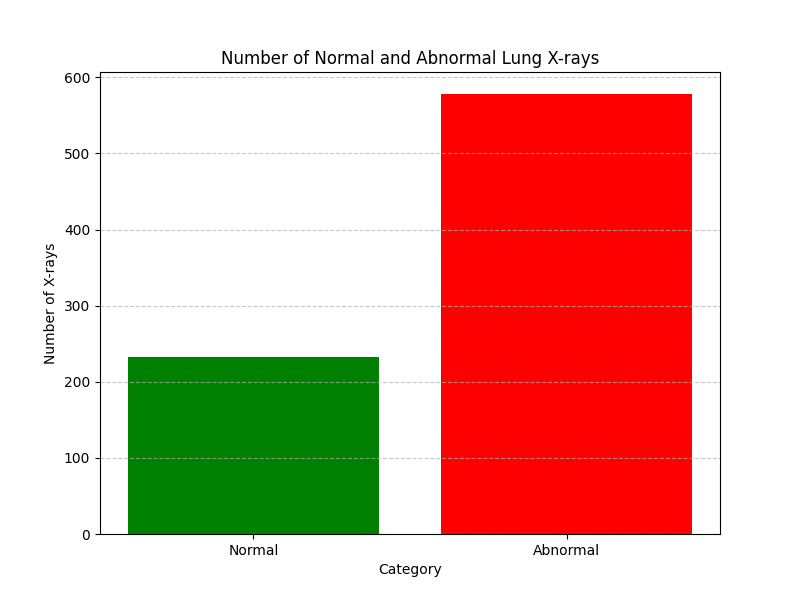
\includegraphics[scale=0.405]{normal_vs_abnormal}
    \caption{The distribution of normal vs. abnormal lung X-rays}
    \label{fig:normalvabnormal}
\end{figure}

As shown in Figure \ref{fig:datasetdistribution}, there is a very clear class imbalance, with "None"
and "Atelectasis" occuring the most and "Pneumonia" and "Hernia" occuring the least. 

%%% DATASET DISTRIBUTION FIGURE -- wide image, so must appear across both columns %%%
\begin{figure*}[!h]
    \centering
    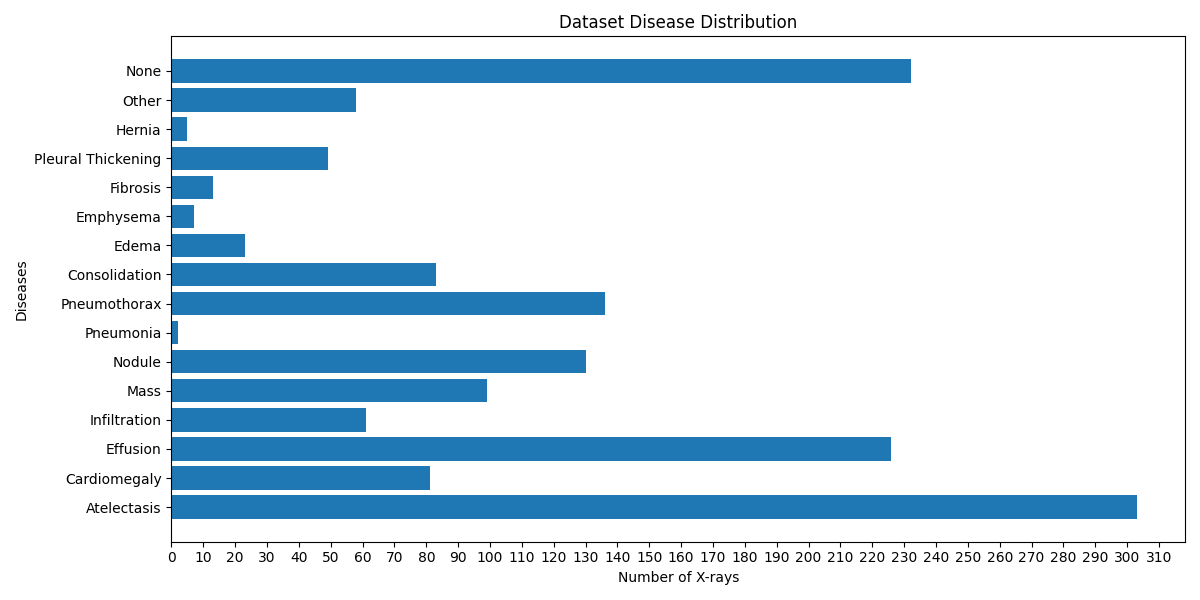
\includegraphics[scale=0.55]{disease_distr}
    \caption{The disease distribution of the dataset with Diseases vs. Number of X-rays.
    As shown, there are 15 labels, including the "None" label. The class imbalance can also be seen.}
    \label{fig:datasetdistribution}
\end{figure*}

%%%%%%%%%%%%%%%%%%%%%%%%%%%%%%%%
% METHODS
%%%%%%%%%%%%%%%%%%%%%%%%%%%%%%%%

\section{Methods}
Three separate models were used in order to accomplish this project. The first was a Support Vector
Machine (SVM) model whereas the other two relied on Convolutional Neural Networks (CNN) in the form
of ResNet50 and MobileNet. The data was split into a 60\% training, 20\% testing, and 20\% validation
separation. Section \ref{section:svm} describes the Support Vector Machine model while Section
\ref{section:cnn} explains the different Convolutional Neural Networks that were used.

\subsection{Support Vector Machine}
\label{section:svm}
Support Vector Machine or SVM is a supervised machine learning model used to separate classes based
on their ability to be separated linearly. The class instances are graphed and ideally separated
into clusters. SVM models take this data and create a linear separator that creates the maximum
margin between clusters. In the case where a linear separator is not successful, the model can employ
the kernel trick, which adds higher dimensions in order to create a substantial margin between classes.
SVMs are less prone to overfitting compared to some algorithms like neural networks, making them
effective for image classification tasks.

The SVM model used specifically classified between Normal and Abnormal classes. The images were first
resized to a fixed shape and flattened into a 1D array. These resized images, along with their labels,
were converted into a Pandas dataframe, and then split into the previously mentioned 60:20:20 split.
The base of the SVM model was taken from the sklearn library in Python, with GridSearchCV for
hyperparameter optimization (C, gamma, kernel).

\subsection{Convolutional Neural Networks}
\label{section:cnn}
Convolutional Neural Networks or CNN are a type of neural network that are designed to process images.
Neural networks are machine learning models that use artificial neurons, or nodes, to process data.
Each node takes in the weights of each feature, computes the sum, and runs it through an activation
function. The activation function can be any function, such as ReLU or the sigmoid function. 

CNNs differ from neural networks by containing a convolutional layer, which takes in input data,
a filter, and a feature map. The convolutional layer takes a group of pixels and applies the filter
to them, boiling them down to a single value. This allows for the given images to reduce in size and
promotes better feature selection. 

\subsubsection{ResNet50}
ResNet50 is a type of CNN that is part of the Residual Networks family. The number 50 indicates that
the model has 50 different layers, including convolution layers, convolution blocks, residual blocks,
and fully connected layers. It has been pre-trained on the large-scale ImageNet dataset and is
well-suited for extracting high-level image features (patterns such as edges, textures, and objects). 

This specific model was only trained and tested on a handful of diseases, as opposed to the entire
set of labels. In the ResNet50 model that was used for this project, the base layers were frozen in order to make
use of the image extraction features of the model, whereas the top layers were trained on the X-ray
dataset. The top layers used ReLU activation, L2 regularization, and dropout and global
average pooling, which reduced feature maps to scalers. This model was trained with the Adam optimizer
to adjust learning rate during training. The loss function associated with ResNet50 was binary
cross-entropy loss.

\subsubsection{MobileNet}
MobileNet, similarly to ResNet50, is a CNN that is capable of image classification. However,
MobileNet is significantly less complex than ResNet50 and attempts to reach similar levels of
accuracy with less parameters and more optimizations. Due to its similarity, it also uses convolution
layers and has been pre-trained on the ImageNet dataset. Additionally, for this model, both the Normal/Abnormal
classes and the multi-label classification were tested.

Again, similarly to ResNet50, the MobileNet model used in this project had top layers that used ReLU
activation, L2 regularization, and global average pooling. The output layer used sigmoid activation
for multi-label predictions. It was also trained with the Adam optimizer with applied image
augmentation (rotation, shift, zoom, flip, etc.) using ImageDataGenerator. The loss function was also
binary cross-entropy loss.

%%%%%%%%%%%%%%%%%%%%%%%%%%%%%%%%
% RESULTS
%%%%%%%%%%%%%%%%%%%%%%%%%%%%%%%%

\section{Results}
In this section, the efficacy of all three models alongside further insights will be discussed.
Due to the differences in the models, the SVM model was tested slightly differently than the two CNN
models, which only have a precision score and not an accuracy percentage.
In Section \ref{section:resultsvm}, the SVM model results will be explored. In Sections
\ref{section:resultresnet50} and \ref{section:resultmobilenet}, both the ResNet50 and MobileNet
models will be reviewed.

\subsection{Support Vector Machine}
\label{section:resultsvm}
As previously mentioned, the SVM model was only used to differentiate between Normal and Abnormal
classes as it was computationally very expensive. Training the model took a substantial amount of
time, even with only two classes, likely due to the fact that SVM is not necessarily designed to
process images, unlike the other two models.

Using the sklearn accuracy\_score() metric, the accuracy of the model without any normalization was
approximately 75\% [Fig \ref{fig:confusionmatrix1}].

%%% CONFUSION MATRIX WITHOUT NORMALIZATION %%%
\begin{figure}[!h]
    \centering
    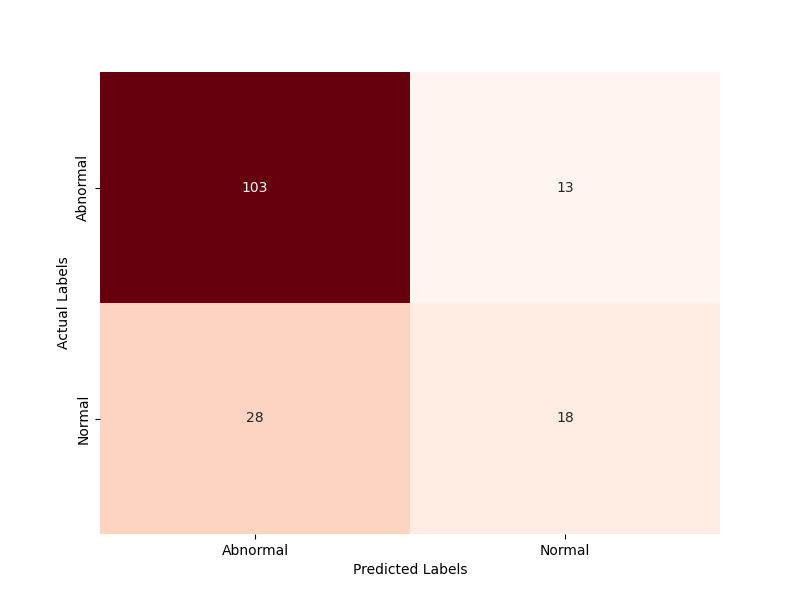
\includegraphics[scale=0.405]{confusion_matrix}
    \caption{The confusion matrix for the SVM model \textbf{without} normalization ($\sim$75\% accuracy).}
    \label{fig:confusionmatrix1}
\end{figure}

With normalization, the accuracy surprisingly dropped to 73\% [Fig \ref{fig:confusionmatrix2}].

%%% CONFUSION MATRIX WITH NORMALIZATION %%%
\begin{figure}[!h]
    \centering
    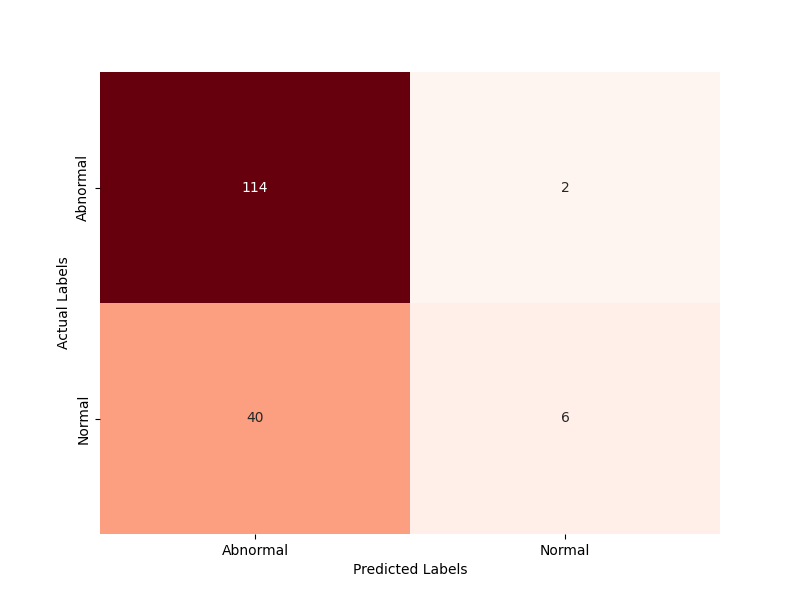
\includegraphics[scale=0.405]{confusion_matrix2}
    \caption{The confusion matrix for the SVM model \textbf{with} normalization ($\sim$73\% accuracy).}
    \label{fig:confusionmatrix2}
\end{figure}

Table \ref{table:svmaccuracy} highlights the precision, recall, and F1-scores of the SVM model.
The model succeeded in predicting the Abnormal class significantly better than the Normal class,
meaning it generally overpredicted diseases and produced many false positives.

%%% PRECISION, RECALL, AND F1 SCORES OF SVM %%%
\begin{table}[!h]
    \centering
    \begin{tabular}{ c  c  c  c }
        \hline
        \textbf{Class} & \textbf{Precision} & \textbf{Recall} & \textbf{F1-Score} \\
        \hline
        Abnormal & 0.79 & 0.89 & 0.83 \\
        Normal & 0.58 & 0.39 & 0.47 \\
        \hline
    \end{tabular}
    \caption{The precision, recall, and F1-scores of the SVM model.}
    \label{table:svmaccuracy}
\end{table}

The biggest limitation to this model was how expensive it is to train, even when boiling the data
down into Normal and Abnormal classes. This means that the model could most likely never be used for
complete image classification including all of the possible labels without employing many
optimizations. This model also does not account for the class imbalance issue. Since the multi-label
capability was not tested in this model, it cannot be determined whether a kernel trick would be
necessary or not. 

\subsection{ResNet50}
\label{section:resultresnet50}
The ResNet50 model was trained and tested only on the diseases: Atelectasis, Consolidation,
Effusion, Mass, Nodule, Pleural Thickening, and Pneumothorax. These were the most frequent diseases
in the dataset, allowing the model to be trained on slightly more balanced data. Table
\ref{table:resnet50accuracy} shows the precision, recall, F1-scores, and support of all labels
using the ResNet50 model. The support value is measured based on the number of examples in each set. 
As expected, the model more accurately predicted diseases that appeared more often. 

%%% PRECISION, RECALL, F1 SCORES, AND SUPPORT OF RESNET50 %%%
\begin{table}[!h]
    \centering
    \resizebox{\columnwidth}{!}{
    \begin{tabular}{ c  c  c  c  c }
        \hline
        \textbf{Class} & \textbf{Precision} & \textbf{Recall} & \textbf{F1-Score} & \textbf{Support}\\
        \hline
        Abnormal & 0.85 & 1.00 & 0.92 & 136 \\
        Atelectasis & 0.64 & 1.00 & 0.78 & 103 \\
        Consolidation & 0.51 & 1.00 & 0.68 & 82 \\
        Effusion & 0.43 & 1.00 & 0.60 & 69 \\
        Mass & 0.75 & 0.09 & 0.16 & 34 \\
        Nodule & 0.34 & 1.00 & 0.51 & 55 \\
        Pleural Thickening & 0.42 & 0.91 & 0.58 & 68 \\
        Pneumothorax & 0.33 & 0.76 & 0.46 & 37 \\
        \hline
    \end{tabular}
    }
    \caption{The precision, recall, F1-scores, and support of the ResNet50 model, where support is
    the number of examples/diseases in the set.}
    \label{table:resnet50accuracy}
\end{table}

The ResNet50 model generally had high recall amongst almost all of the disease labels, meaning many
true positives were identified. However, given the relatively low precision, the model also
classified many false positives. This model, similar to the SVM model, overpredicted diseases,
regardless of how accurate it was.

ResNet50 likely would also not excel with the entire set of labels, especially given the fact
that the remaining untrained disease labels appear even less often. In the case of further class
balancing, ResNet50 would likely be able to succeed, as it was able to classify the most frequent
classes decently well.

\subsection{MobileNet}
\label{section:resultmobilenet}
Unlike the previous two models, the MobileNet model was trained on the entire set of labels,
including the ability to classify each image with multiple labels. Based on the binary cross-entropy
loss, the accuracy was approximately 89\%. However, in Table \ref{table:mobilenetaccuracy}, the
precision, recall, and F1-scores are significantly lower (mostly at 0) for the labels with little
to no appearances. Again, this is expected since the model will be more likely to assign labels
based on what class has the most instances. Unfortunately, both CNN models suffer from this same
issue, which is likely due to the class imbalance. 

%%% PRECISION, RECALL, F1 SCORES, AND SUPPORT OF MOBILENET %%%
\begin{table}[!h]
    \centering
    \resizebox{\columnwidth}{!}{
    \begin{tabular}{ c  c  c  c  c }
        \hline
        \textbf{Class} & \textbf{Precision} & \textbf{Recall} & \textbf{F1-Score} & \textbf{Support}\\
        \hline
        Atelectasis & 0.64 & 1.00 & 0.78 & 103 \\
        Cardiomegaly & 0.00 & 0.00 & 0.00 & 19 \\
        Consolidation & 0.00 & 0.00 & 0.00 & 22 \\
        Edema & 0.00 & 0.00 & 0.00 & 4 \\
        Effusion & 0.73 & 0.57 & 0.64 & 47 \\
        Emphysema & 0.00 & 0.00 & 0.00 & 0 \\
        Fibrosis & 0.00 & 0.00 & 0.00 & 3 \\
        Hernia & 0.00 & 0.00 & 0.00 & 1 \\
        Infiltration & 0.00 & 0.00 & 0.00 & 10 \\
        Mass & 0.33 & 0.06 & 0.11 & 16 \\
        Nodule & 0.50 & 0.04 & 0.07 & 26 \\
        Normal & 0.57 & 0.41 & 0.48 & 41 \\
        Other & 0.00 & 0.00 & 0.00 & 12 \\
        Pleural Thickening & 0.00 & 0.00 & 0.00 & 18 \\
        Pneumonia & 0.00 & 0.00 & 0.00 & 0 \\
        Pneumothorax & 1.00 & 0.05 & 0.10 & 20 \\
        \hline
    \end{tabular}
    }
    \caption{The precision, recall, F1-scores and support of the MobileNet model, where support is
    the number of examples/diseases in the set.}
    \label{table:mobilenetaccuracy}
\end{table}

In Figure \ref{fig:trainingloss}, the training loss and accuracy are graphed. The training loss and
validation loss decrease over the epochs, which is good for the model. However, since the accuracy
and validation accuracy stay relatively the same, it means that the model is not learning anything
new, even with more training data. This is not very beneficial for the model, since the accuracy
should be increasing overtime. 

\begin{figure}[!h]
    \centering
    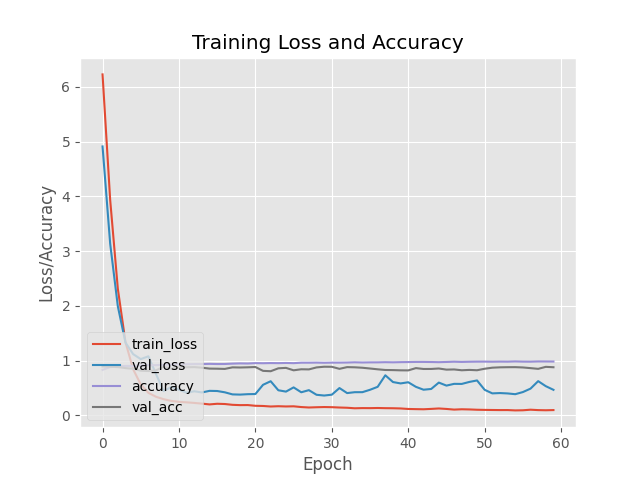
\includegraphics[scale=0.5]{final_results}
    \caption{The plot of Training Loss and Accuracy for multi-label classification.}
    \label{fig:trainingloss}
\end{figure}

Unsurprisingly, the pattern of each model struggling with classifying less frequently seen classes
continues in MobileNet. While the calculated accuracy was certainly quite good, the model just
ignored the labels with less support and did not assign that label to any images, effectively always
getting it wrong, which explains the 0.00 precision, recall, and F1-score of a large chunk of the data.

Overall, this model did perform better than the other two, but there is still much more work to do
in order to have it succeed with this dataset.

%%%%%%%%%%%%%%%%%%%%%%%%%%%%%%%%
% CONCLUSION
%%%%%%%%%%%%%%%%%%%%%%%%%%%%%%%%

\section{Conclusion}
This project demonstrates the potential of machine learning in the medical field, particularly for
diagnosing thoracic disease using patient X-rays. Three models were evaluated by utilizing
X-ray images from the NIH ChestX-ray8 dataset. Starting with an SVM the model was great at
identifying Abnormal cases while it struggled more with Normal cases. This was due to the large
imbalance in data therefore there were few examples that the model could learn from. The SVM
model was also computationally expensive and therefore could not be used for multi-label
classification. However, the CNNs that were developed had better results with the multi-label
classification. ResNet50 demonstrated high recall, identifying many true positives however it
over-predicted diseases leading to overfitting. Finally, the MobileNet was the other CNN that
was utilized and it had the best results, especially with the multi-label classification. MobileNet
achieved an 89\% binary accuracy and was computationally efficient and versatile. For future
implications on this issue, improving data imbalance through oversampling as well as
implementing self-training to obtain more examples could enhance the model’s ability to
generalize and accurately classify diseases.

%%%%%%%%%%%%%%%%%%%%%%%%%%%%%%%%
% CONTRIBUTION CHART
%%%%%%%%%%%%%%%%%%%%%%%%%%%%%%%%



\nocite{jbrownlee}
\nocite{fchollet}
\nocite{mobilenet}
\nocite{svm}
\nocite{tensorflow}
\nocite{athakur}
\nocite{chestx-ray}
\nocite{cnn}

\bibliography{report}
\bibliographystyle{icml2024}

\clearpage
\twocolumn[
\section{Contribution Chart}
Contribution chart listing all group member's contributions.
\newline
]

\begin{table}
    \centering
    \begin{tabular}{| c | c | c | c |}
        \hline
        \textbf{Name} & \textbf{Student ID} & \textbf{Task} & \textbf{Commentary on Contribution} \\
        \hline
        Wendy & 02026116 & SVM and MobileNet & Developed the SVM and MobileNet models. \\ 
        & & & Also, contributed to the slides (specifically the slides \\
        & & & regarding those models) and came up with questions to pose \\
        & & & about the models overall. \\
        \hline
        Meriem & 02015993 & & \\
        \hline
        Chris & 01989716 & & \\
        \hline
        Saim & 02018510 & & \\
        \hline
        Amitha & 02077527 & Research and Report & Created and wrote report. Conducted further research on \\ 
        & & & models and specifications to complete report. Also, contributed to \\
        & & & slides and proposal editing. \\
        \hline
    \end{tabular}
\end{table}

\end{document}
